\lab{Pandas III: Pivot Tables}{Pandas III: Pivot Tables}
\objective{Learn about Pivot tables.}
\label{lab:pandas3}

MAJOR REVISIONS IN PROGRESS!!!!!!!!!!!!!!

\section*{Introduction}
Pandas originated as a wrapper for numpy that was developed by AQR Capital Management, a large investment management company. They used pandas to speed their analysis of financial data. It has since evolved to handle numerous use-cases. Core among its abilities is the power to ``pivot'', or change the main axis of analysis, and then apply functions to that new view. There are two central ways to accomplish this: GroupBy and PivotTables.

\section*{The Titanic Dataset}
We first take a look at how we can use pandas to identify broad trends in the data. We will first look at a simple yet interesting dataset: the Titanic dataset. This dataset contains information (gender, age, class, place of embark, etc.) on passengers from the ill-fated voyage of the Titanic.

\begin{lstlisting}
>>> import numpy as np
>>> import pandas as pd
>>> titanic = pd.read_csv('titanic.csv')
\end{lstlisting}

Let's visualize some of the columns and first couple of rows of our dataset to see what information we can start grouping by to see relations. With this dataset's format, we can just call .head() to visualize the first 5 rows of the table to see what columns are present.

Using the function \li{head()}, we can examine the first few rows of a DataFrame so as to view the columns present.

\begin{lstlisting}
>>> titanic.head()
\end{lstlisting}

Add table
%\begin{figure}
%    \centering
%    \includegraphics[width=.75\textwidth]{heading.pdf}
%\end{figure}

\subsection*{GroupBy()}
Just as it sounds, groupby() takes a DataFrame, and creates groups. The groupby() function does not return anything itself that is helpful to examine. You have to apply some kind of function to the DataFrame object that is returned, but then the function is extremely helpful.

Let's say we want to look at the survival rate of women versus men. How likely was it for a person to survive on the Titanic if they were male as compared to female? We do this with groupby as follows:

\begin{lstlisting}
>>> # Survival rate by gender
>>> titanic.groupby('sex')[['survived']].mean()
\end{lstlisting}

Add table
%\begin{figure}
%    \centering
%    \includegraphics[width=.75\textwidth]{gend_surv.pdf}
%\end{figure}

Here, we chose `sex' as the attribute we want to distinguish the survival rates between. The column `survived' in the titanic dataset contains either a 1 if the passenger survived, or a 0 if they died. Therefore, the survival rate can be found by taking the mean of the entries of the resulting pandas dataframe.

From the table, as we would probably expect, women were more likely to survive than men. But was this true for all different classes on the ship? For example, were women sailing in 1st class more likely to survive than women in 3rd class? In other words, did your class for the voyage have a direct correlation with your survival rate?

We use groupby to help us in the following way:

We pass a list of arguments `sex' and `class', and specify that we want to look at the `survived' values for these different categories. We must then call the aggregate function to organize our data into rows and columns with the value of 'mean' for the intersection of each category. The function unstack() then puts the dataframe into a nice visual format for us.

\begin{lstlisting}
>>> # Survival rate by gender and class. Note how complicated the line is
>>> titanic.groupby(['sex', 'class'])[['survived']].aggregate('mean').unstack()
\end{lstlisting}

Add table
%\begin{figure}
%    \centering
%    \includegraphics[width=.75\textwidth]{gend_class.pdf}
%\end{figure}

Note how long of a function call this previous groupby statement was. Because this functionality is used so often, pandas was built to include a much more quick and efficient way to make these types of tables - pivot tables!

Reorder this.

\subsubsection*{Groupby}
Many datasets are simply composed of tables of individuals, with a list of classifiers associated with each one.
Data like this is difficult to sensibly plot in its raw format.

For example, consider the \li{msleep} dataset (found in \li{pydataset}). 
Each row consists of a single type of mammal and its corresponding identifiers, including genus and order, as well as sleep measurements such as total amount of sleep (in hours) and REM sleep, in hours.
When we try to plot this data using plt.plot, the individual data points do not demonstrate overall trends.
\begin{lstlisting}
>>> msleep = data("msleep")
>>> msleep.plot(y="sleep_total", title="Mammalian Sleep Data", legend=False)
>>> plt.xlabel("Animal Index")
>>> plt.ylabel("Sleep in Hours")
>>> plt.show()
\end{lstlisting}
The above code results in Figure 11.
\begin{figure}[H] 
    \centering
    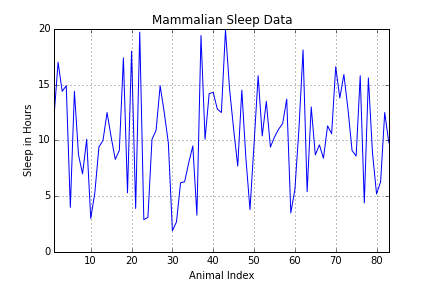
\includegraphics[width=.75\textwidth]{Msleep1.png}
    \caption{Source:  Proceedings of the National Academy of Sciences, 104 (3):1051-1056, 2007. Updates from V. M. Savage and G. B. West, with additional variables supplemented by Wikipedia.}
    \label{fig:aplot}
\end{figure}
This seemingly random set of connected data points is not particularly revealing.

We thus decide to approach our dataset using pandas' powerful \li{groupby} method. 
Let's say that, for the \li{msleep} dataset, we want to visualize the differences in sleep data between herbivores, omnivores, insectivores and carnivores.
Then, we simply call the groupby method on the \li{vore} column to obtain a groupby object organized diet classification.
\begin{lstlisting}
>>> msleep = data("msleep")
>>> vore = msleep.groupby("vore")
\end{lstlisting}
You can also group the data by multiple columns, for example, both the \li{vore} and \li{order} classifications.
To group and view this data, simply use:
\begin{lstlisting}
>>> vorder = msleep.groupby(["vore", "order"])

# View groups within vorder
>>> vorder.describe
\end{lstlisting}

Pandas \li{groupby} objects are not lists of new dataframes associated with groupings.
They are better thought of as a dictionary or generator-like object which can be \emph{used} to produce the necessary groups.
However, if you want to work within a dataframe for a specific group, you may use the \li{get\_group()} method as follows:

\begin{lstlisting}
# Get carnivore group
>>> Carni = vore.get_group("carni")
# Get herbivore group
>>> Herbi = vore.get_group("herbi")
\end{lstlisting}

The \li{groupby} object includes many useful methods that can help us make visual comparisons between groups. 
The \li{mean()} method, for example, returns a new dataframe consisting of the mean values attached to each group.
For example, using this method on our \li{vore} object returns a nicely organized dataframe of the average sleep data for each mammalian diet pattern.
We can similarly create a dataframe of the standard deviations for each group.

At this point, we have a nicely organized dataset that can easily be turned into a bar chart.
Here, we use the \li{dataframe.loc} method to access three specific columns in the bar chart (\li{sleep_total}, \li{sleep_rem}, and \li{sleep_cycle}).
\begin{lstlisting}
>>> means = vore.mean()
>>> errors = vore.std()

>>> means.loc[:,["sleep_total", "sleep_rem", "sleep_cycle"]].plot(kind="bar", yerr=errors, title="Mean Mammallian Sleep Data")
>>> plt.xlabel("Mammal diet classification (vore)")
>>> plt.ylabel("Hours")
>>> plt.show()
\end{lstlisting}

\begin{figure}[H] 
    \centering
    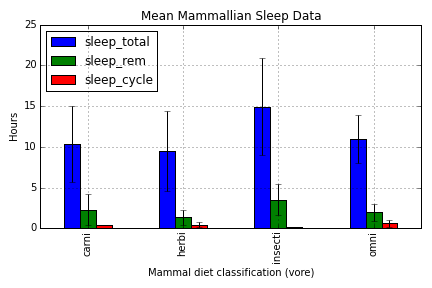
\includegraphics[width=.75\textwidth]{MeanMammal.png}
    \caption{Source:  Proceedings of the National Academy of Sciences, 104 (3):1051-1056, 2007. Updates from V. M. Savage and G. B. West, with additional variables supplemented by Wikipedia.}
    \label{fig:aplot}
\end{figure}

The pandas \li{groupby} object has many different methods.
We have discussed a few of these here; for more information please see: 
\begin{itemize}
    \item \url{http://pandas.pydata.org/pandas-docs/stable/generated/pandas.DataFrame.groupby.html}
    \item \url{http://pandas.pydata.org/pandas-docs/stable/groupby.html}
\end{itemize}

\begin{problem} 
Examine the \li{diamonds} dataset found in the \li{pydataset} module. 
This dataset contains the identifiers and attributes of 53,940  individual round cut diamonds. 
Using the \li{groupby} method, create three different visuals highlighting and comparing different aspects of the data.
This can be in the form of a single plot or comparative subplots.

Print a few sentences for each plot explaining what type of graph you used, why, and what we learn about the dataset from your plot.
Don't forget that points will be taken off for each plot without a title, clear labels, and sourcing. 
\end{problem}

The following is an example of the kind of plot we are looking for. 
This example may not be used as one of your three plots.
\begin{figure}[H] % Matplotlib vs. Pandas
    \centering
    \begin{minipage}[b]{0.48\textwidth}
    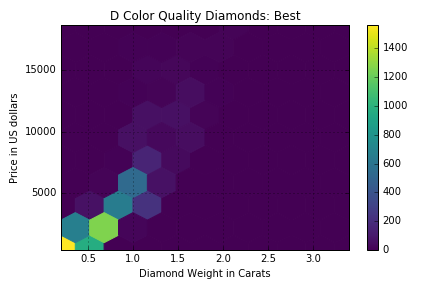
\includegraphics[width=\textwidth]{DiamondD.png}
    \end{minipage}
    \quad
    \begin{minipage}[b]{0.48\textwidth}
    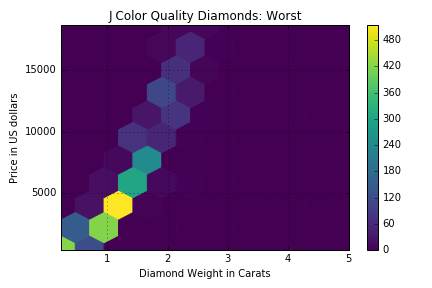
\includegraphics[width=\textwidth]{DiamondJ.png}
    \end{minipage}
    \caption{Source: Adopted from R Documentation}
    \label{fig:intro2}
\end{figure}

The code for the above figure is included here:
\begin{lstlisting}
>>> Diamonds = data("diamonds")
>>> DiaColor = Diamonds.groupby("color")
>>> Ddiamond = DiaColor.get_group("D")
>>> Jdiamond = DiaColor.get_group("J")

>>> Ddiamond.plot(kind="hexbin", x="carat", y="price", gridsize=10, title="D Color Quality Diamonds: Best", cmap="viridis")
>>> plt.ylabel("Price in US Dollars")
>>> plt.xlabel("Diamond Weight in Carats")
>>> plt.tight_layout()
>>> plt.show()

>>> Jdiamond.plot(kind="hexbin", x="carat", y="price", gridsize=10, title="J Color Quality Diamonds: Worst", cmap="viridis")
>>> plt.ylabel("Price in US Dollars")
>>> plt.xlabel("Diamond Weight in Carats")
>>> plt.tight_layout()
>>> plt.show()
\end{lstlisting}

We now analyze the plots.

The above plots were created using \li{groupby} on the diamond colors and then using a hexbin comparing carats to price for the highest and lowest quality diamonds, respectively. 
This hexbin is particularly revealing for each set of thousands of diamonds because it meaningfully displays concentration of datapoints. 
Matplotlib's new \li{viridis} colorplot, with a dark background, reveals bins that would have been invisible with a white background.
By comparing these plots, we note that the greatest number of J quality diamonds in the dataset are about 1.25 carats and \$4000 dollars in price, whereas the highest concentration of D quality diamonds are smaller and therefore cheaper. 
We may attribute this to D quality diamonds being rarer, but the colorbar on the side reveals that D diamond numbers are, in fact, far higher than those of the J color. 
Instead it is simply more likely that D quality diamonds of larger sizes are rarer than those of smaller sizes. 
Both hexbins reveal a linearity between diamond weight and diamond price, with D diamonds showing more variability and J diamonds displaying a strict linearity.

\section*{Pivot Tables}
With a given pandas dataframe, we can visualize all of these tables easily with the function \li{pivot_table()}. To accomplish basically the same task as before of comparing the survival rates for both genders and each class, we can call:

\begin{lstlisting}
>>> # We can do the same thing, with less code in df.pivot_table()
>>> titanic.pivot_table('survived', index='sex', columns='class')
\end{lstlisting}

Add table
%\begin{figure}
%    \centering
%    \includegraphics[width=.75\textwidth]{piv_gend_class.pdf}
%\end{figure}

Here ``value'' is the category (or column in the original datset) we want to compare, ``index'' will be the category for the row of our pivot table, and ``columns'' is the category to organize as the columns for our pivot table.

Let's say we want to further break down the survival rates to compare how different ages fared in the voyage, according to their gender and class. We could be asking ourselves the question, ``What about the children? Were male children really that likely to die as compared to female children?''. As you will see with pivot tables, as we see these simple breakdowns of the data, more questions can, and should arise. You should consistently ask yourself questions about the relevance of the numbers you see in the pivot tables you create. So let's look at how age was a factor in survival.

Noting that in the original dataset, the `age' column has an integer value for the age of each passenger, if we were to just add `age' as an argument for index, then the table would create a new row for EACH age present. This wouldn't be a very useful or simple table to visualize, so we desire to partition the ages into 3 categories. We use the function \li{cut()} to do this.

\begin{lstlisting}
>>> # Partition each of the passengers into 3 categories based on their age
>>> age = pd.cut(titanic['age'], [0,12,18,80])
\end{lstlisting}

Now with this other partition of the column age, we can add this dimension to our pivot table, passing it along with `sex' in a list to the parameter index.

\begin{lstlisting}
>>> # Add a third dimension, age, to our pivot table
>>> titanic.pivot_table('survived', index =['sex', age], columns='class')
\end{lstlisting}

Add table
%\begin{figure}
%    \centering
%    \includegraphics[width=.75\textwidth]{piv_gend_class_age.pdf}
%\end{figure}

What do we notice? First of all, male children (ages 0 to 12) in 1st and 2nd class were very likely to survive, whereas those in 3rd class did not. However, look at the female children in first class. 0 percent of them survived? This might seem a little odd, but if we looked at our data set again to see how many passengers fell into this category of female, 1st class, and age 0 to 12, we would find only 1 passenger. Therefore, the statistic that 0\% of female children in first class died is misleading. We can visualize this by specifying the parameter aggfunc=`count'.

\begin{lstlisting}
>>> titanic.pivot_table('survived', columns='sex', index=['class',age], aggfunc='count')
\end{lstlisting}

Add table
%\begin{figure}
%    \centering
%    \includegraphics[width=.75\textwidth]{piv_gca_count.pdf}
%\end{figure}

The parameter aggfunc defaults to `mean', which is why we have seen the mean survival rate for each of the different categories. By specifying aggfunc to be `count', we get how many passengers of each category are present in the table. In this case, specifying the value is `survived' is redundant.

This brings up another point about these datasets. We note for this dataset, we have roughly 800 passengers' data. This is not that large of a data set relatively, and we aren't guaranteed significant sample sizes for each possible partitioning of the the data columns. This is important to keep in mind with any dataset, and you should always ask questions about the numbers you see in pivot tables before making any conclusions.

Now, for fun, let's add a fourth dimension to our table- the cost of the passenger's ticket. Let's add this dimension to our columns of the pivot table. We now use the function \li{qcut()} to partition the fare column's data into two different categories.

With this partition we add this dimension to columns, passing fare and `class' in as a list to the argument ``columns".

\begin{lstlisting}
>>> # Partition fare column into 2 categories based on the values present in fare column
>>> fare = pd.qcut(titanic['fare'], 2)
>>> # Add the fare as a dimension of columns
>>> titanic.pivot_table('survived', index=['sex',age], columns=[fare, 'class'])
\end{lstlisting}

Add table
%\begin{figure}
%    \centering
%    \includegraphics[width=.75\textwidth]{fare_splice.pdf}
%\end{figure}

We now see something else about our dataset - we get NaNs in some entries. The dataset has some invalid entries or incomplete data for the column fare. Let's investigate further.

By inspecting our dataset, we can see that there might not be any people in the categories given in the pivot table. We can fill in the NaN values in the pivot table with the argument \li{fill_value}. We show this below.

\begin{lstlisting}
>>> # Specify fill_value = 0.0
>>> titanic.pivot_table('survived', index=['sex',age], columns=[fare, 'class'], fill_value=0.0)
\end{lstlisting}

Add table
%\begin{figure}
%    \centering
%    \includegraphics[width=.75\textwidth]{fill_zeros.pdf}
%\end{figure}

It should be noted though that with datasets where NaN's occur frequently, some preprocessing needs to be done so as to get the most accurate statistics and insights about your dataset. You should've worked on cleaning datasets in previous lab, so we don't go further into detail about the topic here.

\begin{problem}
Suppose that someone claims that the city from which a passenger embarked had a strong influence on the passenger's survival rate. Investigate this claim.
\begin{enumerate}
\item Using a \li{groupby()} call, see what the survival rates of the passengers were based on where they embarked from (\li{embark_town}).
\item Next, create a pivot table to further look at survival rates based on both place of embarkment and gender.
\item What do these tables suggest to you about the significance of where people embarked in influencing their survival rate? But in light of the context of the problem, what do you think this really means? Find 2 more pivot tables that investigate the claim further, looking at other criterion (e.g., class, age, etc.).
\end{enumerate}
\end{problem}












